\frame{\tableofcontents[sectionstyle=show/hide,subsectionstyle=show/show/hide]}

\subsection{SMS}
\begin{frame}
    \frametitle{\currentsectionname}
    \begin{enumerate}
        \item Bestätigungscode wird als SMS-Nachricht gesendet
        \item Eingabe des Codes in App
    \end{enumerate}
    \begin{itemize}
        \item am weitesten verbreitet
        \item einige Usability- und Sicherheitsprobleme, aber einfaches Setup
    \end{itemize}

    \note{
        Usability-Probleme:
        \begin{itemize}
            \item verzögerte Zustellung
            \item kein Empfang
            \item Fehler bei Eingabe des Codes
        \end{itemize}
        Sicherheits-Probleme:
        \begin{itemize}
            \item keine Verschlüsselung -> Man In The Middle
            \item SIM-Swapping
            \item Server muss Code sicher speichern
            \item Brute-Force Angriffe sind nicht ausgeschlossen
        \end{itemize}
    }
\end{frame}

\subsection{TOTP}
\begin{frame}
    \frametitle{\currentsectionname}
    \begin{enumerate}
        \item Nutzer scannt QR-Code, Scanner generiert Bestätigungscode
        \item Bestätigungscode wird eingegeben und vom Server überprüft
    \end{enumerate}
    \begin{itemize}
        \item Code hat beschränkte Lebensdauer
        \item Spezieller Scanner oder Smartphone benötigt
    \end{itemize}

    \note{
        \begin{itemize}
            \item benötigt kein Internet oder Netz \textrightarrow{} weniger Angriffsfläche
        \end{itemize}
        Usability:
        \begin{itemize}
            \item relative kompliziertes Setup
            \item nicht alle haben Smartphone
            \item Fehler bei Eingabe des Codes
        \end{itemize}
        Sicherheit:
        \begin{itemize}
            \item Verschlüsselung \textrightarrow{} besser als SMS
            \item Server und Client müssen Code sicher speichern
        \end{itemize}
    }
\end{frame}

\subsection{Vor-Generierte Codes}
\begin{frame}
    \frametitle{\currentsectionname}
    \begin{itemize}
        \item Liste von Codes wird vorgeneriert
        \item ca.\ acht Zeichen lang
        \item Codes müssen sicher aufbewahrt werden
    \end{itemize}

    \note{
        \begin{itemize}
            \item Länge der Codes lädt zu Fehlern bei Aufbewahrung / Eingabe ein
            \item Server und Nutzer müssen Codes sicher aufbewahren
            \item Keine Kontrolle über Sicherheit der Aufbewahrung auf Nutzerseite
            \item Codes sehr lange / immer gültig \textrightarrow{} empfänglich für Brute Force
        \end{itemize}
    }
\end{frame}

\subsection{Push Benachrichtigungen}
\begin{frame}
    \frametitle{\currentsectionname}
    \begin{enumerate}
        \item Nutzer erhält Benachrichtigung auf Smartphone
        \item Möglichkeit Login-Versuch zu bestätigen oder abzulehnen
    \end{enumerate}
    \begin{itemize}
        \item Benötigt Smartphone und meist spezifische App
        \item Keine Eingabe von Code benötigt
    \end{itemize}

    \note{
        \begin{itemize}
            \item Server muss Benachrichtigung an richtiges Gerät schicken
            \item kein Code \textrightarrow{} weniger fehleranfällig
            \item könnte als nutzerfreundlicher und schneller empfunden werden
        \end{itemize}
    }
\end{frame}

\subsection{U2F Sicherheitsschlüssel}
\begin{frame}
    \frametitle{\currentsectionname}
    \begin{columns}
        \begin{column}{0.7\textwidth}
            \begin{itemize}
                \item \textit{Universal 2nd Factor (U2F)}:
                    offener Standard für Authentifizierung durch ein Security-Token
                \item Nutzer muss Token an PC anschließen und aktivieren,
                    sobald App dazu auffordert
                \item Server speichert öffentlichen Schlüssel
                \item Security-Token speicher geheimen Schlüssel
            \end{itemize}
        \end{column}
        \begin{column}{0.3\textwidth}
            \begin{figure}
                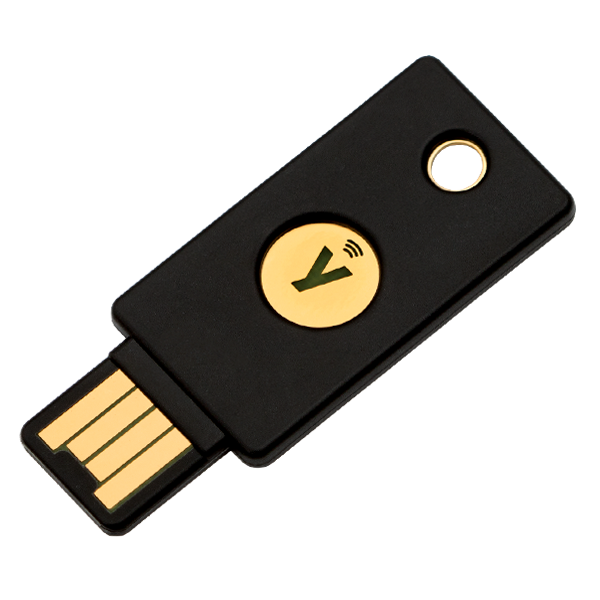
\includegraphics[height=\linewidth]{ubikey}
                \caption{YubiKey\endnote{\url{https://media.yubico.com/media/catalog/product/5/n/5nfc_hero_2021.png}}}
            \end{figure}
        \end{column}
    \end{columns}

    \note{
        \begin{itemize}
            \item wurde als sehr sichere, und trotzdem nutzerfreundliche Methode konzipiert
            \begin{itemize}
                \item[\textrightarrow] deshalb besonders interessant, wie Nutzer dies empfinden
            \end{itemize}
            \item Sicherheitsrisiko: Verlieren des USB Sticks
            \begin{itemize}
                \item[\textrightarrow] besteht allerdings auch bei anderen Methoden
            \end{itemize}
        \end{itemize}
    }
\end{frame}
